\documentclass{article}
% Include all project wide packages here.
\usepackage{fullpage}
\usepackage{polyglossia}
\setmainlanguage{dutch}
\usepackage{csquotes}
\usepackage{graphicx}
\usepackage{epstopdf}
\usepackage{pdfpages}
\usepackage{caption}
\usepackage[list=true]{subcaption}
\usepackage{float}
%\usepackage{mathtools}
\usepackage{standalone}
\usepackage{import}
\usepackage{tocloft}
\usepackage{wrapfig}
\usepackage{authblk}
\usepackage{array}
\usepackage{booktabs}
\usepackage[toc,page,title,titletoc]{appendix}
\usepackage{xunicode}
\usepackage{amsmath}
\usepackage{fontspec}
\usepackage{unicode-math}
\usepackage[
    backend=bibtexu,
	texencoding=utf8,
bibencoding=utf8,
    style=ieee,
    sortlocale=nl_NL,
    language=auto
]{biblatex}
\usepackage{listings}
\newcommand{\includecode}[3][c]{\lstinputlisting[caption=#2, escapechar=, style=#1]{#3}}
\newcommand{\superscript}[1]{\ensuremath{^{\textrm{#1}}}}
\newcommand{\subscript}[1]{\ensuremath{_{\textrm{#1}}}}


\newcommand{\chapternumber}{\thechapter}
\renewcommand{\appendixname}{Bijlage}
\renewcommand{\appendixtocname}{Bijlagen}
\renewcommand{\appendixpagename}{Bijlagen}

\usepackage[hidelinks]{hyperref} %<--------ALTIJD ALS LAATSTE

\renewcommand{\familydefault}{\sfdefault}

\setmainfont[Ligatures=TeX]{Myriad Pro}
\setmathfont{Asana Math}
\setmonofont{Lucida Console}

\usepackage{titlesec, blindtext, color}
\definecolor{gray75}{gray}{0.75}
\newcommand{\hsp}{\hspace{20pt}}
\titleformat{\chapter}[hang]{\Huge\bfseries}{\chapternumber\hsp\textcolor{gray75}{|}\hsp}{0pt}{\Huge\bfseries}
\renewcommand{\familydefault}{\sfdefault}
\renewcommand{\arraystretch}{1.2}
\setlength\parindent{0pt}

%For code listings
\definecolor{black}{rgb}{0,0,0}
\definecolor{browntags}{rgb}{0.65,0.1,0.1}
\definecolor{bluestrings}{rgb}{0,0,1}
\definecolor{graycomments}{rgb}{0.4,0.4,0.4}
\definecolor{redkeywords}{rgb}{1,0,0}
\definecolor{bluekeywords}{rgb}{0.13,0.13,0.8}
\definecolor{greencomments}{rgb}{0,0.5,0}
\definecolor{redstrings}{rgb}{0.9,0,0}
\definecolor{purpleidentifiers}{rgb}{0.01,0,0.01}


\lstdefinestyle{csharp}{
language=[Sharp]C,
showspaces=false,
showtabs=false,
breaklines=true,
showstringspaces=false,
breakatwhitespace=true,
escapeinside={(*@}{@*)},
columns=fullflexible,
commentstyle=\color{greencomments},
keywordstyle=\color{bluekeywords}\bfseries,
stringstyle=\color{redstrings},
identifierstyle=\color{purpleidentifiers},
basicstyle=\ttfamily\small}

\lstdefinestyle{c}{
language=C,
showspaces=false,
showtabs=false,
breaklines=true,
showstringspaces=false,
breakatwhitespace=true,
escapeinside={(*@}{@*)},
columns=fullflexible,
commentstyle=\color{greencomments},
keywordstyle=\color{bluekeywords}\bfseries,
stringstyle=\color{bluestrings},
identifierstyle=\color{purpleidentifiers}
}

\lstdefinestyle{vhdl}{
language=VHDL,
showspaces=false,
showtabs=false,
breaklines=true,
showstringspaces=false,
breakatwhitespace=true,
escapeinside={(*@}{@*)},
columns=fullflexible,
commentstyle=\color{greencomments},
keywordstyle=\color{bluekeywords}\bfseries,
stringstyle=\color{redstrings},
identifierstyle=\color{purpleidentifiers}
}

\lstdefinestyle{xaml}{
language=XML,
showspaces=false,
showtabs=false,
breaklines=true,
showstringspaces=false,
breakatwhitespace=true,
escapeinside={(*@}{@*)},
columns=fullflexible,
commentstyle=\color{greencomments},
keywordstyle=\color{redkeywords},
stringstyle=\color{bluestrings},
tagstyle=\color{browntags},
morestring=[b]",
  morecomment=[s]{<?}{?>},
  morekeywords={xmlns,version,typex:AsyncRecords,x:Arguments,x:Boolean,x:Byte,x:Char,x:Class,x:ClassAttributes,x:ClassModifier,x:Code,x:ConnectionId,x:Decimal,x:Double,x:FactoryMethod,x:FieldModifier,x:Int16,x:Int32,x:Int64,x:Key,x:Members,x:Name,x:Object,x:Property,x:Shared,x:Single,x:String,x:Subclass,x:SynchronousMode,x:TimeSpan,x:TypeArguments,x:Uid,x:Uri,x:XData,Grid.Column,Grid.ColumnSpan,Click,ClipToBounds,Content,DropDownOpened,FontSize,Foreground,Header,Height,HorizontalAlignment,HorizontalContentAlignment,IsCancel,IsDefault,IsEnabled,IsSelected,Margin,MinHeight,MinWidth,Padding,SnapsToDevicePixels,Target,TextWrapping,Title,VerticalAlignment,VerticalContentAlignment,Width,WindowStartupLocation,Binding,Mode,OneWay,xmlns:x}
}

%defaults
\lstset{
basicstyle=\ttfamily\small,
extendedchars=false,
numbers=left,
numberstyle=\ttfamily\tiny,
stepnumber=1,
tabsize=4,
numbersep=5pt
}



\begin{document}
De beschrijving van de opdrachtgevers hebben we verder geïnterpreteerd in VHDL-code. Hieronder worden de verschillende aspecten van het ontwerp besproken. 
%Beschrijf hoe de beschrijving van de opdrachtgevers verder geïnterpreteerd is en hoe het ontwerp gedaan is, tot aan de %VHDL beschrijving.
\begin{itemize}
\item Eerst is gekeken wat een Alu is en wat hij eigenlijk doet. Daaruit kwam naar voren dat het een soort calculator is, die berekeningen met - of operaties op - bits uitvoert.  Daarbij is in ons geval het aantal bits de parameter. (zie Specificaties)

\item Daarna  is men begonnen met het schrijven van een entity (appendix \ref{entity}) met alle in en uitgangen en een behaviour hierbij. Dit wordt hieronder uitgewerkt.  
\end{itemize}
\subsection{Blokrepresentatie met in- en uitgangen}
Het systeem wordt weergegeven in figuur \ref{1}. 
\begin{figure} [h!]
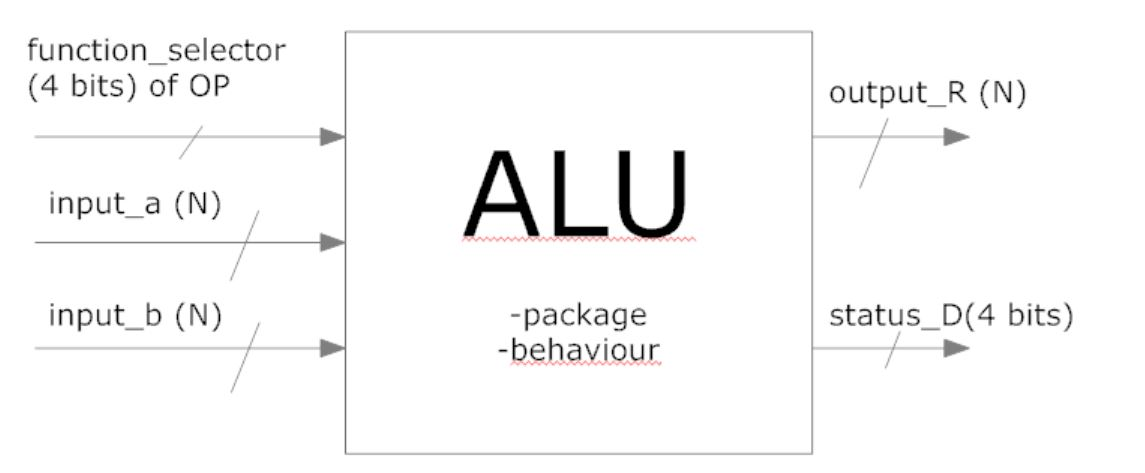
\includegraphics [scale = .4]{figures/blk}
\caption{Het blokschema van de Alu}
\label{1}
\end{figure}
De Alu wordt bediend door de Op-code, een 4 bits signaal. De ingangssignalen zijn input\_a en input\_b met een variabel aantal bits N. Die wordt als parameter meegegeven aan de Alu. (te zien aan het woord "package") Vervolgens wordt de berekening uitgevoerd in behaviour VHDL. Stel dat er een carry ontstaat, dan wordt signaal status\_D 0001. Stel dat er een zero ontstaat (bij and-operatie), dan wordt status\_D 0010. Hier zou je op aan kunnen merken dat je lang niet zoveel status\_D signalen nodig hebt en dus ook een 2-bit\_vector zou aan kunnen maken. Wellicht is dit gedaan omdat later complexere alu's meer uitgangscontrolesignalen nodig zijn. De berekende waarde wordt weergegeven aan output\_R
met als lengte de waarde van de parameter. De parameter heet in ons programma S. 
\subsection{Een of meerdere toestandsdiagrammen }
We hebben niet echt een toestandsdiagram, maar in de VHDL-code in \ref{behaviour} kun je precies zien wat er gebeurd als de opcode veranderd of niet gedefinieerd is. 
\subsection{VHDL behaviour beschrijving van de schakeling}
De behaviour beschrijving staat in appendix \ref{behaviour}. Bovenaan staan de nodige singalen. Dan wordt een process gestart met Op in de sensitivity list. Als variabelen in de sensitivity list veranderen, verandert ook de uitgang. In dit geval zorgt een verandering in Op voor een andere output (behalve als bij een Op geen operatie bestaat, dan komt hij in de default (when others) terecht, waarbij de uitgang en de status\_D allebei nul worden). Uiteindelijk wordt Reg3 gelijkgemaakt aan output\_R. 
\subsection{Simulatieresultaten van de VHDL behaviour beschrijving}
\begin{figure} [h!]
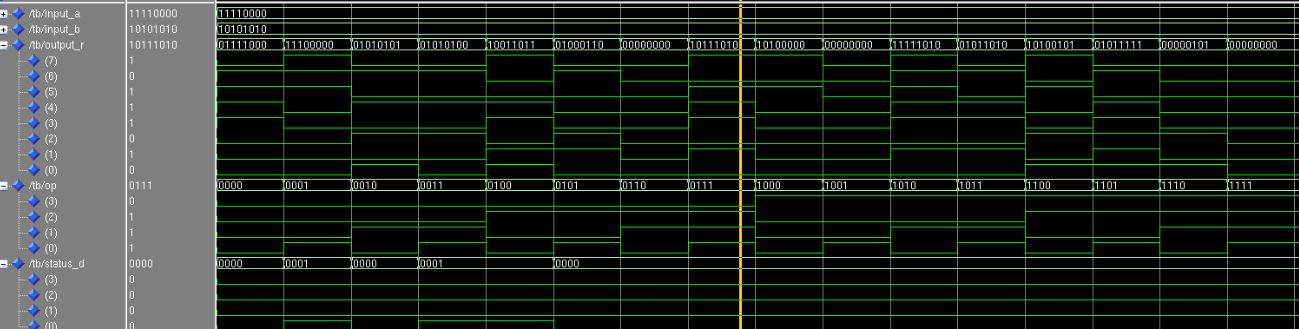
\includegraphics [scale = .35]{figures/simtb}
\caption{Het simulatieresultaat van de alu}
\label{2}
\end{figure}
Nadat de behaviour uitvoerig gecompileerd is, is er een testbench geschreven (appendix \ref{tb}). Daarna zijn er configuraties aangemaakt in GoWithTheFlow. Vervolgens werd de simulatie gestart. In figuur \ref{2} staat het resultaat.
Eerst klopte deze simulatie nog niet. Het bleek namelijk dat de carry niet werd meegenomen. Dat is aangepast in de behaviour, waarna de carry wel werd meegenomen. Nu worden input\_a en input\_b een S+1 bits signaal gemaakt, waarna na een operatie wordt gechekct of het MSB 1 is. Is dat het geval, dan is er een carry ontstaan en wordt status\_D 0001.  Dit is overeenkomstig de specificaties. De rest van de VHDL-simulatie is ook gecontroleerd en goed bevonden. 

\end{document}